% Options for packages loaded elsewhere
\PassOptionsToPackage{unicode}{hyperref}
\PassOptionsToPackage{hyphens}{url}
%
\documentclass[
  11pt,
]{article}
\usepackage{amsmath,amssymb}
\usepackage{lmodern}
\usepackage{iftex}
\ifPDFTeX
  \usepackage[T1]{fontenc}
  \usepackage[utf8]{inputenc}
  \usepackage{textcomp} % provide euro and other symbols
\else % if luatex or xetex
  \usepackage{unicode-math}
  \defaultfontfeatures{Scale=MatchLowercase}
  \defaultfontfeatures[\rmfamily]{Ligatures=TeX,Scale=1}
\fi
% Use upquote if available, for straight quotes in verbatim environments
\IfFileExists{upquote.sty}{\usepackage{upquote}}{}
\IfFileExists{microtype.sty}{% use microtype if available
  \usepackage[]{microtype}
  \UseMicrotypeSet[protrusion]{basicmath} % disable protrusion for tt fonts
}{}
\makeatletter
\@ifundefined{KOMAClassName}{% if non-KOMA class
  \IfFileExists{parskip.sty}{%
    \usepackage{parskip}
  }{% else
    \setlength{\parindent}{0pt}
    \setlength{\parskip}{6pt plus 2pt minus 1pt}}
}{% if KOMA class
  \KOMAoptions{parskip=half}}
\makeatother
\usepackage{xcolor}
\usepackage[left = 2.5cm, right = 2cm, top = 2cm, bottom =
2cm]{geometry}
\usepackage{graphicx}
\makeatletter
\def\maxwidth{\ifdim\Gin@nat@width>\linewidth\linewidth\else\Gin@nat@width\fi}
\def\maxheight{\ifdim\Gin@nat@height>\textheight\textheight\else\Gin@nat@height\fi}
\makeatother
% Scale images if necessary, so that they will not overflow the page
% margins by default, and it is still possible to overwrite the defaults
% using explicit options in \includegraphics[width, height, ...]{}
\setkeys{Gin}{width=\maxwidth,height=\maxheight,keepaspectratio}
% Set default figure placement to htbp
\makeatletter
\def\fps@figure{htbp}
\makeatother
\setlength{\emergencystretch}{3em} % prevent overfull lines
\providecommand{\tightlist}{%
  \setlength{\itemsep}{0pt}\setlength{\parskip}{0pt}}
\setcounter{secnumdepth}{5}
\usepackage{float}
\usepackage{sectsty}
\usepackage{paralist}
\usepackage{setspace}\spacing{1.5}
\usepackage{fancyhdr}
\usepackage{lastpage}
\usepackage{dcolumn}
\usepackage{natbib}\bibliographystyle{agsm}
\usepackage[nottoc, numbib]{tocbibind}
\ifLuaTeX
  \usepackage{selnolig}  % disable illegal ligatures
\fi
\IfFileExists{bookmark.sty}{\usepackage{bookmark}}{\usepackage{hyperref}}
\IfFileExists{xurl.sty}{\usepackage{xurl}}{} % add URL line breaks if available
\urlstyle{same} % disable monospaced font for URLs
\hypersetup{
  hidelinks,
  pdfcreator={LaTeX via pandoc}}

\author{}
\date{\vspace{-2.5em}}

\begin{document}

\allsectionsfont{\centering}
\subsectionfont{\raggedright}
\subsubsectionfont{\raggedright}

\pagenumbering{gobble}

\begin{centering}

\vspace{3cm}


\includegraphics[width=0.2\linewidth]{FHCW_logo} 

\includegraphics[width=0.2\linewidth]{KI_logo} 

\vspace{1cm}

\Large
\doublespacing
{\bf Design and implementation of analysis pipeline for single cell type proteomics data} 

\vspace{1 cm}

\normalsize
\singlespacing
By

\vspace{0.5 cm}

\Large

{\bf Lukas Gamp}

\vspace{1.5 cm}

in partial fullfilment of the requirement \\for the degree of MSc \\in Bioinformatics

\vspace{1.5 cm}

\normalsize
mm yy
\end{centering}

\newpage

\pagenumbering{gobble}

\begin{centering}

{\bf Abstract}

\end{centering}

\spacing{1.5}

(the spacing is set to 1.5)

no more than 250 words for the abstract

\begin{itemize}
\tightlist
\item
  a description of the research question/knowledge gap -- what we know
  and what we don't know
\item
  how your research has attempted to fill this gap
\item
  a brief description of the methods
\item
  brief results
\item
  key conclusions that put the research into a larger context
\end{itemize}

\pagenumbering{roman}

\newpage

\centering
\raggedright
\newpage
\tableofcontents

\newpage

\section*{Acknowledgements}

Thank you for following this tutorial!

I hope you'll find it useful to write a very professional dissertation.

\newpage

\hypertarget{introduction}{%
\section{Introduction}\label{introduction}}

\hypertarget{proteomics}{%
\subsection{Proteomics}\label{proteomics}}

The proteome is referred to the sum of all proteins of a given sample at
a given time. In the past several quantitative and qualitative assays
were used to enlighten the protein composition of a sample.

An early approach of qualitative analysis of the cellular proteome
involved labeling with fluorescent antibodies and imaging. The major
disadvantage of this technique was the limitation to only stain a few
proteins per cell. For quantification procedures such as single-cell
Western blots, immunoassays or CyTOF have been used. Other disadvantages
are the ability to permeate cells, accessibility and binding of the
epitope and the creation of specific antibodies for a given protein
\citep{Budnik2018}.

One of those techniques involved RNA-sequencing. Since RNA involves also
non-coding RNA, the amount of RNA is often not proportional to the
content of proteins in a cell. So the proteinaceous content of a cell
was only predicted and quantitative analysis was not possible.

\hypertarget{mass-spectrometry}{%
\subsection{Mass Spectrometry}\label{mass-spectrometry}}

Mass spectrometry enables qualitative and quantitative analysis of the
entire repertoire of a biological sample. The availability of gene
sequences in databases and the ability to match proteins against those
sequences with computational methods makes it possible to identify
alterations of a sample on a protein level. These alterations can rely
on the sequence level or could be to post-translational modifications
(PTMs) such as phosphorylation, methylation or else
\citep{Aebersold2003}.

Mass to charge ratio (m/z)

\pagenumbering{arabic}

\newpage

\hypertarget{materials-and-methods}{%
\section{Materials and Methods}\label{materials-and-methods}}

\hypertarget{materials}{%
\subsection{Materials}\label{materials}}

For analysis two types of cells were used. One type is the Jurkat-based
cell line (J-lat) with integrated HIV.

The other type of cells are macrophages with a sample size of 72 cells.
The analysis is done with two groups. A HIV negative (HIV-) control
group and a HIV positive (HIV+) group.

\hypertarget{cell-isolation}{%
\subsubsection{Cell Isolation}\label{cell-isolation}}

\hypertarget{lysis}{%
\subsubsection{Lysis}\label{lysis}}

\hypertarget{digestion}{%
\subsubsection{Digestion}\label{digestion}}

\hypertarget{labeling-techniques}{%
\subsubsection{Labeling techniques}\label{labeling-techniques}}

For differential analysis proteins need to be labeled to compare mass to
charge intensities in order to quantify observed peptides. Since mass
spectrometry is not a quantitative technique by itself, the peak height
or area does not reflect the abundance of a peptide. Physicochemical
properties of the proteins can change the ionization efficiency and
detectability of the target. However, when comparing the same analyte
between multiple runs of labeled proteins, differences in the mass
spectrum reflect the abundance of those. Labels should be chosen to
change solely the mass of the sample and to not affect folding or other
inherent properties of the protein.

\hypertarget{metabolic-labeling}{%
\paragraph{Metabolic labeling}\label{metabolic-labeling}}

Feeding cells with aminoacids containing heavy isotopes, is the method
of choice in order to label peptides at the earliest possible level.
This atoms can be heavy nitrogen in aminoacids or salts in fertilizer
for plants. Mass shifts are proportional to the isotopes incorporated
during biomass production and are visible after proteolytic cleavage.
Stable isotope labeling in cell culture (SILAC) was presented in the
early 2000s. This method used heavy aminoacid enriched media to feed
cells, in order to quantitatively analyze expression profiles.

\hypertarget{isobaric-labeling}{%
\paragraph{Isobaric labeling}\label{isobaric-labeling}}

\hypertarget{tandem-mass-tag-tmt}{%
\subparagraph{Tandem mass tag (TMT)}\label{tandem-mass-tag-tmt}}

Tandem mass tag (TMT) reagents enable to differentiate multiple samples
analyzing in one MS run. The samples are labeled individually and pooled
afterwards, this procedure is called multiplexing. TMTs have the same
charge and differ only by their isotopic masses, the peaks found for
each sample are called reporter ions (RI). Each RI and sample is
interpreted as one channel in downstream analysis. The identification of
these RI leads to an enrichment and identification of low abundance
peptide ions which is common especially in single-cell techniques. With
this technique it is possible to quantify proteins and differ low
abundant proteins from background noise. The disadvantage of isobaric
labeling is, that the co-fragmentation signals can be observed in the
spectrogram and the data needs to be normalized in order to remove
unwanted contribution \citep{Marx2019, Budnik2018}. Furthermore TMTs
have an isotopic distribution according to the distribution found in
nature. This can be corrected during data-acquisition as a defined
spread in other channels.

\hypertarget{instrumentation}{%
\subsubsection{Instrumentation}\label{instrumentation}}

\hypertarget{liquid-chromatography}{%
\paragraph{Liquid chromatography}\label{liquid-chromatography}}

In order to separate proteins according to their chemical properties,
size or species a liquid chromatography (LC) is recommended before
ionization.

\hypertarget{mass-spectrometry-1}{%
\paragraph{Mass Spectrometry}\label{mass-spectrometry-1}}

\hypertarget{ionization}{%
\subparagraph{Ionization}\label{ionization}}

In order to analyze a biological sample consisting of proteins in
solution the liquid needs to be vaporized into gas phase. Two techniques
are capable of this procedure. Electrospray ionization (ESI) pushes the
analyte through a capillary and applies an electric current to the
liquid, vaporizing the sample to a charged aerosol. Biomolecules are
fragmented according to their chemical properties and can be further
handled in the mass spectrometer. The fragmented biomolecules are now in
charged droplets separated by their charge on the surface, splitting
further into smaller droplets until they become a gas phase ion. Two
physical models describe the process from gas phase to ion called ``The
ion evaporation model'' (IEM) and ``The charge residue model'' (CRM). In
the ion evaporation model (by Iribarne and Thomoson) the droplets shrink
by evaporation until ions are expelled. The model had its limitation by
explaining same evaporation rate constant among ions with different
chemical properties. In the charge residue model the assumption of one
molecule per droplet leads to an ionization rate constant, which is
independent of the ion itself and relies solely on the generation of the
droplet and the efficiency of the solvent \citep{Wilm2011}.

Matrix-assisted laser desorption/ionization (MALDI)

\hypertarget{ms.1}{%
\subparagraph{MS.1}\label{ms.1}}

\hypertarget{coupled-mass-spectrometry-msms-ms.2}{%
\subparagraph{Coupled mass-spectrometry (MS/MS) \&
MS.2}\label{coupled-mass-spectrometry-msms-ms.2}}

In order to enhance sequence identification, two MS devices are built in
series. In the first run (MS1) the m/z is determined and the molecules
are passed to the next device. Upon passing the molecules are fragmented
into smaller ions and analyzed by the second MS. The fragmentation
highly depends on the chemical bonds found in the molecule. The majority
of these breaks occur on the peptide bond of the protein, although this
is not guaranteed for all bonds and so it can happen that certain
peptide ions have a low abundance \citep{Budnik2018}. These low abundant
peptides will not be detected, hence the problem needs to be faced with
another approach . A solution for this problem is molecular barcoding
with labeling mentioned in the chapter labeling.

\hypertarget{data}{%
\subsection{Data}\label{data}}

\hypertarget{acquisition}{%
\subsubsection{Acquisition}\label{acquisition}}

Acquisition of the data was done with MaxQuant \citep{Cox2008} software
package.

\hypertarget{ms-spectrum}{%
\paragraph{MS-Spectrum}\label{ms-spectrum}}

Each peptide is reflected by its` indivual fingerprint in the
ms-spectrum. The fingerprint is based on the chemical properties and
modifications of aminoacids. These aminoacids can be calculated through
their m/z ration and after that interpreted as an aminoacid sequence.
Due to fragmentation of the protein only peptide sequences are visible
in the spectrum. In order to identify proteins, peptides are matched
against a sequence database \citep{Cox2008}. Sequence Databases are
simple .fasta files, which can be downloaded on the uniprot webpage
(www.uniprot.org).

Since ms data has a high resolution, algorithms are used to convert the
raw signal to an interpretable form. MaxQuant is one of many sofware
packages to process the data and provides it for further analysis and
statistical testing. Other software solutions are Protein Discoverer
Thermo Fisher or even packages for R. In this publication we will mainly
focus on the data-acquisition with MaxQuant \citep{Cox2008}.

\hypertarget{three-dimensional-peak-detection}{%
\paragraph{Three-dimensional peak
detection}\label{three-dimensional-peak-detection}}

The three dimensions of the data are: m/z ratio, intensity and retention
time. The algorithm finds local minima of the function in order to
seperate peaks from each other. The centroid of the peak is detected by
fitting a so called gaussian peak shape fitting. This can be interpreted
as finding the peaks of each m/z spectrum as a function of time.. The
centroid of the peak refers to an isotope.

\hypertarget{deisotoping}{%
\paragraph{Deisotoping}\label{deisotoping}}

To decrypt the istopic distribution of a biomolecule, MaxQuant creates a
vertex of every single peak and connects them with their possible
isotopic counterparts by finding the proportion of mass of an average
aminoacid to its` respective isotope (averagine \citep{Senko1995}).
Isotoping is the term of such procedure and it is enabled with graph
theory. After this procedure the amount of data points are reduced by a
tenfold and a single peak reflects a small biomolecule.

\hypertarget{label-detection}{%
\paragraph{Label detection}\label{label-detection}}

The next step in data-acquisition is the detection of labels for
quantification. Isotopic pairs of the label (e.g.~N13, N14, N15)
contained in the tag or aminoacid can be identified by convoluting the
two measured isotope patterns with the theoretical isotope patterns.
With a least-square method the best fit is found iteratively and the
channel/sample can be identified.

\hypertarget{improving-peptide-mass-accuracy}{%
\paragraph{Improving peptide mass
accuracy}\label{improving-peptide-mass-accuracy}}

The intensity-weighted average of the ms peak centroids (as described in
the 3D peak identification) refers to the mass of the peptide.
Corrections highly depend on the analyzer, MaxQuant uses for an orbitrap
typed analyzer a correction value of 1ppm. Autocorrelation between
centroids is compensated by only using well-identified peptides. As
published the mass precision within a ms experiment ranges around 10e-7.

\hypertarget{peptide-search}{%
\paragraph{Peptide search}\label{peptide-search}}

Biomolecules can now be searched in a database in forward and reverse
direction. The peptide identification (P-) score indicates the fit of
the data to the found sequence in the database according to the length
of the peptide and is used to calculate the posterior error probability
(FDR). The calculation of the false discovery rate is then calculated by
taking FDR into contrast.

\hypertarget{protein-assembly}{%
\paragraph{Protein assembly}\label{protein-assembly}}

After these calculation the identified peptides can be aggregated
according to it`s respective protein and quantified. The mentioned
metrics indicating the performance of the peptide search can be used in
downstream analysis. A so called razor peptide indicates the group with
the highest number of identified peptides. Quantification is enabled by
taking only unique peptides into contrast. Posterior error
probabilities, which refers to the chance that the found peptide is a
random event, are multiplied and only distinct sequences with the
highest-scoring are used.

\hypertarget{data-processing}{%
\subsubsection{Data processing}\label{data-processing}}

Further analysis is done with R and respective packages such as
bioconductor. Since there is no state of the art established, analysis
varies upon experimental design. The workflow of the analysis will be
processed in a so called pipeline streamlining the data through steps
where individual results can be observed in visualizations and indivdual
calculations will be adapted according to user demands and experimental
properties.

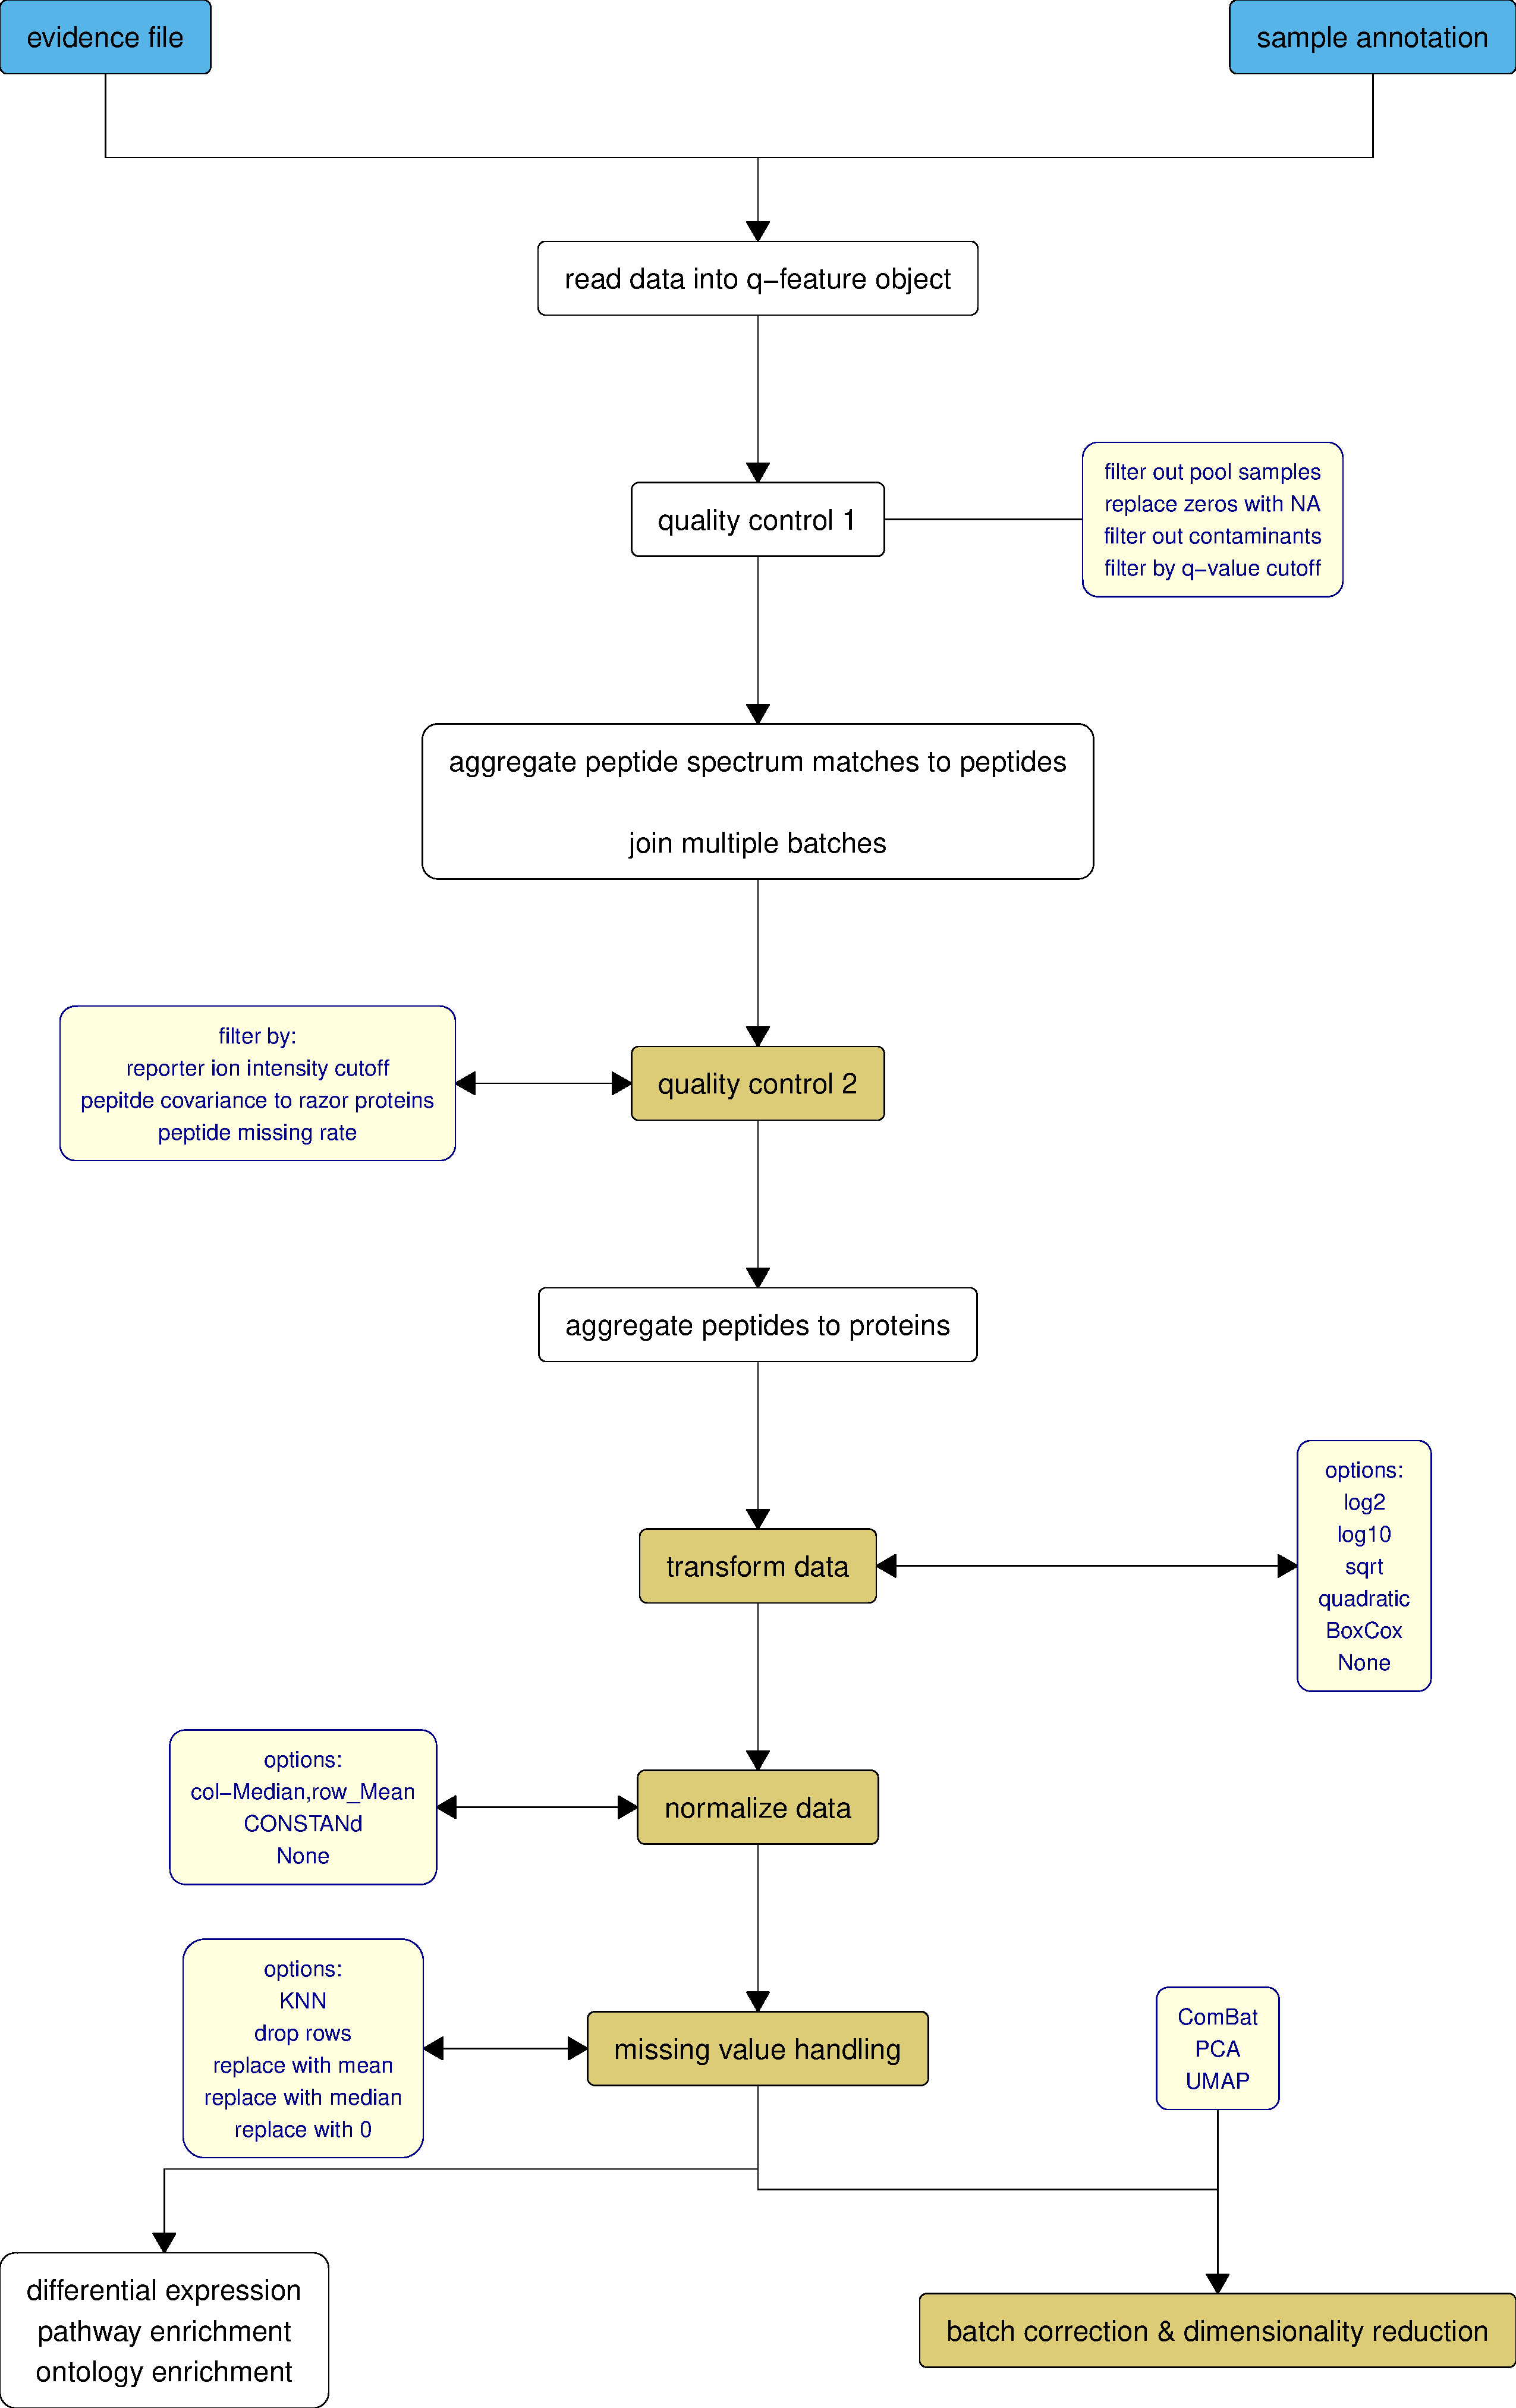
\includegraphics{Thesis_files/figure-latex/data_processing_pipeline_flowchart_vertical-1.pdf}

\hypertarget{reading-the-data}{%
\paragraph{Reading the data}\label{reading-the-data}}

After processing MaxQuant creates a directory containing all results as
.txt file. The evidence.txt file include all peptide to spectrum matches
(PSM) with their respective proteins and statistical parameters.

Example fo basic parameters and derivations include:

\begin{itemize}
\tightlist
\item
  Peptide sequence
\item
  Mass to charge ratio (m/z) for all scans (eg. MS1, MS2)

  \begin{itemize}
  \tightlist
  \item
    Mass
  \end{itemize}
\item
  Retention time
\item
  Precursor Ion Fragment

  \begin{itemize}
  \tightlist
  \item
    source of the detected ion also referred as mother ion
  \end{itemize}
\item
  Fraction of total spectrum
\item
  Base peak fraction
\item
  Reporter intensity (RI)

  \begin{itemize}
  \tightlist
  \item
    corrected RI
  \end{itemize}
\item
  Posterior error probability (PEP)
\end{itemize}

\hypertarget{object-oriented-programming}{%
\paragraph{Object oriented
programming}\label{object-oriented-programming}}

In order to streamline the analysis of multiple experiments, object
oriented programming can be applied. The approach in R is to create a so
called Q-feature object, which contains all variables and metadata in a
hierarchical structure. The structure enables sub setting for further
analysis \citep{Vanderaa2021}.

\hypertarget{zero-values}{%
\paragraph{Zero values}\label{zero-values}}

Peptides with low abundance are often set to zero during analysis.
However, assigning a value of zero may incorrectly suggest that the
sample does not contain the respective peptide. Given that it is highly
unlikely for a biological cell of a comparable type and function to not
contain a particular protein, replacing the zero value with ``not
applicable'' (NA) is crucial for understanding and interpreting MS data.

\hypertarget{exclude-reverse-matchescontaminants}{%
\paragraph{Exclude reverse
matches/contaminants}\label{exclude-reverse-matchescontaminants}}

Peptide sequences matching to the reverse protein sequences (=decoy
database) are considered as possible contaminants. These matches can be
excluded from further analysis.

\hypertarget{filter-according-to-precursor-ion-fraction-pif}{%
\paragraph{Filter according to precursor ion fraction
(PIF)}\label{filter-according-to-precursor-ion-fraction-pif}}

During mass spectrometry, the ions detected in MS1 are further
fragmented through collision during multiple MS runs. The resulting
product ions are derived from precursor ions (also known as mother ions
or parental ions). Contaminant peptides can co-migrate in this process
and can be distinguished by the lower fraction of their respective
precursor ions \citep{Tannous2020}. These peptides need to be filtered
out during the analysis pipeline. A cutoff value, referenced in the
SCoPE2 pipeline \citep{Specht2021}, is applied in the user interface,
but it can be adjusted according to the needs of the biologist.

\hypertarget{filter-by-q-value}{%
\paragraph{Filter by q-value}\label{filter-by-q-value}}

The next step for quality control is the exclusion of samples with a
high false discovery rate (FDR). When applying multiple statistical
testing (e.g.~t-Test) the obtained p-values can be considered as biased,
because the probability to observe a significant will iteratively
increase with each test performed. Corrections in statistics are an
approach to compensate for the multiplicity of testing. There are many
ways to do this compensation like the Bonferroni method or
Benjamini-Hochberg`s FDR. In Mass spectrometry the common ``way to go''
is calculating a false discovery rate, by dividing false PSMs (=hit of
the decoy database) through the total number of PSMs above the
peptide-spectrum matching score. The peptides spectrum matching score is
defined as -10log10(p). Whereas the p-value is defined that the hit is
done by chance. The calculation of the score is highly dependent on the
data acquisition method used. MaxQuant uses Andromeda , an integrated
search engine. Proteome Discoverer from Thermo Fisher utilizes different
engines such as Mascot or Minora. As published by J.Cox in 2011 Mascot
and Andromeda showed similar performance when comparing FDR values as a
function of coverage. However the observed performance can be lower when
dealing with a decreased coverage \citep{Cox2011}.The threshold for
accepting an FDR of an individual PSM is described as q-value.

\hypertarget{peptide-spectrum-match-psm-aggregation-to-peptides}{%
\paragraph{Peptide spectrum match (PSM) aggregation to
peptides}\label{peptide-spectrum-match-psm-aggregation-to-peptides}}

In data science, aggregation refers to a row-wise operation that merges
data based on a particular column using a specific function. In the
context of processing from peptides to spectrum matches, the desired
column is the peptide sequence. To account for different distributions
across multiple assays, the median of the channel is used as the
function to aggregate multiple matches into one.

\hypertarget{join-assays-when-observing-multiple-comparable-batches-at-once}{%
\paragraph{Join assays when observing multiple comparable batches at
once}\label{join-assays-when-observing-multiple-comparable-batches-at-once}}

Sample size is often a limiting factor in hypothesis testing. A strict
quality control and the fact that TMT reagents are only available up to
18-plex can reduce the number of observed samples below the critical
threshold, leading to an early end of analyses. To overcome this
limitation, the provided software is capable of processing multiple runs
simultaneously, allowing for testing of multiple batches and increasing
the number of samples that can be included in the analysis.

\hypertarget{calculate-reporter-ion-intensity-ri-and-filter-according-to-median-ri}{%
\paragraph{Calculate reporter ion intensity (RI) and filter according to
median
RI}\label{calculate-reporter-ion-intensity-ri-and-filter-according-to-median-ri}}

Columns which do not meet the desired intensity can be filtered by a
threshold set on the RI. The median RI can also be used to check if an
entire channel has a lower detection level. This can be due two reasons.
One is the expression level of the given proteins in a cell. Meaning,
that the expression of the observed cell type is simply lower than the
other type. Another one could be a spillage of TMT detection in other
channels due incorrect or missing correction of the TMT isotopes.

\hypertarget{calculate-and-filter-according-to-median-coefficient-of-variation-cv-per-cellchannel}{%
\paragraph{Calculate and filter according to median coefficient of
variation (CV) per
cell/channel}\label{calculate-and-filter-according-to-median-coefficient-of-variation-cv-per-cellchannel}}

Depending having a bulk sample or single-cell sample choosing a minimum
of observed peptides and a cutoff value for the CV, changes the level of
confidence in the peptide data. The coefficient of variation of a
peptide is considered as the ratio of the standard deviation to the mean
and describes the relationship of the observed peptide signal over
multiple proteins (=razor proteins). Peptides having a high coefficient
of variation over many razor proteins are considered as noise and need
to be filtered out before statistical analysis.

\hypertarget{remove-peptides-with-high-missing-rate}{%
\paragraph{Remove peptides with high missing
rate}\label{remove-peptides-with-high-missing-rate}}

Although missing value imputation can be performed during the analysis
of multiple batches, peptides with missing detections across channels
can be problematic for quantification. The proteomic composition of a
biological sample is similar between replicates and even across groups.
However, the threshold of missingness (described as a fraction of the
row) can be set in the user interface and adjusted to enable different
experimental designs.

\hypertarget{aggregation-of-peptides-to-proteins}{%
\paragraph{Aggregation of peptides to
proteins}\label{aggregation-of-peptides-to-proteins}}

Similar to the already explained previous aggregation step the peptides
will be further processed into their respective proteins after the
quality control on the peptide level is performed. Finally an expression
matrix for every protein and their respective channel column is
returned. Each channel refers to a sample and reflects contains the
intensities of each protein found in the biological specimen.

\hypertarget{transformation-of-protein-expression-data}{%
\paragraph{Transformation of protein expression
data}\label{transformation-of-protein-expression-data}}

Data transformation applies a function to each value of a matrix or
array, so that: \[
y_i = f(x_i)
\] Depending on the distribution of the values in the observed
expression set, different transformations can be applied to fulfill
assumptions for statistical testing. In the shiny application, various
procedures are implemented and can be further expanded upon request from
the user. The macrophage analysis done by Specht et al.~mentioned in
their SCoPE2 publication \citep{Specht2021} uses the logarithm to the
base 2 to spread a compacted distribution and remove skewness in the
dataset. This transformation was used as a reference when comparing
methods. However, using the logarithm to the base 10 may be an easily
interpretable way of defining expression data and will also be
facilitated by other transformation methods such as the boxcox method,
which is also implemented in the application. When observing a wide
distribution of small and large values of the expression set in a
histogram, a square root transformation can help increase the
variability of smaller values and decrease the variability of larger
values. Practically impossible, but in data-driven science, occasionally
negative expression values may be present, and they can be converted
into positive values by taking each one to the power of two. Depending
on the distribution, the user has to decide which transformation to
consider and verify that statistical assumptions are met after
application with visualizations such as histograms, qqplots, and
MA-plots. For statistically inexperienced users, the boxcox
transformation can help with this decision. Developed in 1964 by Box and
Cox \citep{Sakia1992}, this method applies a linear model against 1 on
the data to determine the statistical parameter lambda by the maximum
likelihood method. The log-likelihood method takes the 95\% confidence
interval for the parameter lambda and the final lambda is chosen as the
value with the highest log-likelihood value.

\begin{center}
\begin{tabular}{l r}
$\lambda$ & Transformation \\
-2 & $\frac{1}{x^2}$ \\
-1 & $\frac{1}{x}$ \\
-0.5 & $\frac{1}{\sqrt{x}}$ \\
0 & $\log{x}$ \\
0.5 & $\sqrt{x}$ \\
1 & $x$ \\
2 & $x^2$
\end{tabular}
\end{center}

Depending on the size of lambda, a certain function will be
automatically applied to each value of the expression set in order to
introduce normality. In terms of usability, the boxcox method is the
most efficient transformation method, taking the decision of which
calculation to apply away from the user.

\hypertarget{normalization}{%
\paragraph{Normalization}\label{normalization}}

The term normalization is ambiguous in data-science and will be
explained briefly in this chapter. Starting with converting the data to
the Z-distribution (Gaussian result), where 0 represents the mean and 1
represents the standard deviation, in vectorization every feature (or
protein) is represented as a vector that points in a specific direction
in the unit sphere, normalization can have different meanings.
Normalization is considered as part of the scaling procedure and ensures
that every feature contributes equally to our statistical model and
hinders large values from biasing the model in a particular direction.
However, this could also have negative consequences for the modeling
procedure, as it may reduce the impact of important features on the
dataset. Depending on the algorithms later used in the data processing,
the method of choice for normalization can change the results
significantly. The K-means clustering algorithm, for instance relies on
the distances between distinct data points by minimizing variance of the
squared euclidean distances. This method will be applied in the missing
value imputation which will be the next step applied to our data.
Therefore, we want to ensure that we obtain the most accurate imputed
values possible. The first normalization method available in the user
interface is column-wise median and row-wise mean normalization. This
method was chosen by Specht et al in the SCoPE2 publication 2021
\citep{Specht2021} and worked as a reference during the development
process to benchmark other methods. When dividing each value of an
expression set by the median of the particular column, the procedure is
considered as a column-wise median normalization. Although the
mean-normalization works the same way but takes the mean as the second
variable. In the analysis pipeline both procedures were applied on the
dataset. However when the logarithm as the transformation method was
chosen as transformation method, the pipeline automatically switches
from a division to a subtraction, since:
\(\log_a \left(\frac{u}{v}\right)=\log_a u-\log_a v\). After applying
this normalization method, each value can be interpreted as a distance
or fraction of the mean or median of the corresponding column or row,
enabling fair comparisons between features and samples. The second
method for normalization included is the CONSTANd method, which was
proven suitable for relative quantification in the field of proteomics
\citep{Maes2016, VanHoutven2021}, but can also be applied on RNAseq
data. CONSTANd uses a technique called matrix raking, which employs the
RAS algorithm. The expression set reflects the nonnegative real
\((m, n)\) matrix \(A\) were the bi proportional constrained matrix
problem will be solved by finding the \((m, n)\) matrix \(B\) which
equals to \(diag(x) * A *diag(y)\) . Whereas \(x \in \mathbb{R}^{m}\)
and \(y \in \mathbb{R}^{n}\). The solution to this problem involves
finding the row sum of \(B=u_i\) and the column sum of \(B=v_j\), where
\(i\) and \(j\) denote the row and column indices of the matrix,
respectively \citep{Bacharach1965}. In other words, the matrix will be
alternatively manipulated on rows and columns until the mean of both
equals 1. In order to apply the method and yield true results, one has
to consider 3 major assumptions between sample types. This assumption
can be observed in the MA-plot which indicates the differences of two
samples. If we have the intensities of two samples, \(R\) and \(G\), we
can plot them on a graph with the x-axis as \(M=\log_2(\frac{R}{G})\)
and the y-axis as \(A=\frac{1}{2}\log_2(RG)\). A comparison between all
sample types of identically processed sets is needed before calculation
and the assumptions must be fulfilled.

\begin{itemize}
\item{\textbf{1}} \textbf{The majority of proteins are not differentially expressed}
\\Density of the dots decreases when looking from the middle of the cloud towards the edges.

\item{\textbf{2}} \textbf{Up- and downregulation is balanced around the mean expression}
\\The scatterplot of the data points is symmetrical around the mean on the horizontal axis. 

\item{\textbf{3}} \textbf{Systematic bias correlates with the magnitude of expression}
\\The symmetry axis is approximately horizontal.

\end{itemize}

If the MA-plot does not visualize any of these violations the CONSTANd
method can be applied on the dataset and the biological meaning of the
sample types can be assessed. The method is utilized by the bioconductor
package handler. However if the dataset already consists of balanced
features and samples or the user wants to benchmark the methods applied,
normalization can be skipped also.

\hypertarget{missing-value-handling}{%
\paragraph{Missing value handling}\label{missing-value-handling}}

When analyzing multiple batches simultaneously, it is possible to
encounter situations where a particular protein is not detected in one
of the batches. From a biological perspective, it is highly unlikely
that a cell completely lacks a single protein, as it would imply a
complete loss of function for that protein. Therefore, an intensity
value of 0 is close to impossible for most proteins. In order to handle
this dark space in the expression set, several methods can be chosen in
the application. A variety of function employs replacing the missing
values with the mean or median of the rest of the matrix. This procedure
introduces no bias in the data if the missingness is low, although
differential expression for the sample carrying the missing feature can
not be expected as well. Even a more conservative approach is dropping
the rows for the feature with the missing value in one of the observed
samples. A common practice in proteomics is utilizing the K-nearest
neighbor algorithm (=KNN), which imputes the missing values by a
euclidean metrics of the neighboring values in the columns where the
feature is not missing. \(K\) denotes for the count of neighboring
values of a gene and can be selected upon preference. The euclidean
distance between two points is defined as \(d = \sqrt{a^2 * b^2}\), the
\(K\) nearest neighbors average value will be assigned to the intensity
of the missing feature. Since the average is a statistical metric which
can be biased easily by skewed distributions, normalization is an
important task before performing missing value imputation. KNN was
benchmarked for the regression of protein abundance intensities and
showed an Area under the Curve (AUC) above 0.7 when testing on a human
proteome test set \citep{Lan2013}.

\hypertarget{batch-correction}{%
\paragraph{Batch correction}\label{batch-correction}}

Since mass spectrometry experiments are highly biased by several
factors, such as sample processing, the technician, manufacturer and
production of the device (chromatography column, mass-spectrometer), the
reagents etc., working in multiple batches introduces further variance
in the protein data. This variance would overshadow the biological
differences across sample types. Before attempting to remove batch
effects it is recommended to elucidate the variance with a
dimensionality reduction technique which will be explained in the next
chapter. To remove the technical factor also called non-biological
experimental variation the R package sva \citep{Leek2012} with the
ComBat function \citep{Johnson2007} was used. The expression of a gene
\(g\) for the batch \(m_i\) and sample \(j\) is defined as
\(Y_i_j_g = a_g + X \beta_g + \gamma_i_g + \delta_i_g \epsilon_i_j_g\),
whereas \(\gamma\) and \(\delta\epsilon\) denote for the systematic
error caused by the batch. In order to remove the systematic error the
bayesian framework shrinks the effect by pooling information over the
features \(g\). Ideally the effects \(a\) and \(\beta\) remain as
natural as they are and should reflect the true biological difference
between experimental obtained samples or groups. ComBat standardizes the
data by a Z-transformation before attempting to remove the batch effect.
By the method of moments the two batch effect parameters \(\gamma\) and
\(\delta\epsilon\) were estimated and can be subtracted from each value
for the particular feature.

\hypertarget{downstream-analysis}{%
\paragraph{Downstream Analysis}\label{downstream-analysis}}

After cleaning the data and crystallizing from impurities such as noise
and unwanted effects, the biological differences between sample types
can be obtained. Proteomic data consists of multi dimensions (=features)
which are overall hard to understand by a glance. An approach to observe
the differences without a closer sight of exact effect on the
proteinaceous ensemble, but still keep a high level of information can
be dimensionality reduction.

\hypertarget{principle-component-analysis-pca}{%
\subparagraph{Principle component analysis
(=PCA)}\label{principle-component-analysis-pca}}

The most common approach in data science for any kind of high
dimensional data is the PCA. Every principle component can be understood
as a vector pointing in a specific direction derived as the eigenvector
from the covariance matrix of the expression set. The covariance matrix
indicates for the co linearity between the variance of all elements
compared. After calculating the covariance matrix the eigenvectors for
the covariance matrix will be obtained by solving the quadratic
equations to obtain the eigenvalues \(\lambda\). Since
\(A v = \lambda v\) the eigenvector \(v\) can be obtained by solving the
equation for each element of the vector. The eigenvectors \(v\) never
changes is direction and explains the covariance within the dataset and
so also the mathematical differences between the samples. The
eigenvectors are sorted according to their eigenvalues in decreasing
order and therefore decreasing explained variance. For graphical
visualizations the principle components are plotted against each other.
The first two components, which explain the majority of variance in the
dateset highlight the difference between samples. After the cleaning
procedures any additional effect caused by technical or biological
replication should be removed, however it could be found be highlighting
according to the particular factor. This makes the PCA to a useful tool
before starting any statistical analysis by checking for involuntarily
introduced bias.

\hypertarget{testing-for-differential-expression}{%
\paragraph{Testing for differential
expression}\label{testing-for-differential-expression}}

In order to test for differential expression the package limma from R
bioconductor was used. \citep{Phipson2016}. The package uses a linear
model approach to define a fold expression between sample groups. Before
starting the analysis two matrices need to be computed. The design
matrix identifies samples according to the sample type and defines the
experimental design. In order to create the matrix automatically a
simple algorithm is used within the programmed backend logic. The
expression matrix contains intensities for each identified protein will
be obtained at the end of the pipeline. A function call with the
arguments design and expression matrix calculates the contrast matrix.
The next step is creating a linear model between groups by log-ratios of
their expression values.

\newpage

\hypertarget{results}{%
\section{Results}\label{results}}

Some more guidlines from the School of Geosciences.

This section should summarise the findings of the research referring to
all figures, tables and statistical results (some of which may be placed
in appendices). - include the primary results, ordered logically - it is
often useful to follow the same order as presented in the methods. -
alternatively, you may find that ordering the results from the most
important to the least important works better for your project. - data
should only be presented in the main text once, either in tables or
figures; if presented in figures, data can be tabulated in appendices
and referred to at the appropriate point in the main text.

\textbf{Often, it is recommended that you write the results section
first, so that you can write the methods that are appropriate to
describe the results presented. Then you can write the discussion next,
then the introduction which includes the relevant literature for the
scientific story that you are telling and finally the conclusions and
abstract -- this approach is called writing backwards.}

\newpage

\hypertarget{discussion}{%
\section{Discussion}\label{discussion}}

the purpose of the discussion is to summarise your major findings and
place them in the context of the current state of knowledge in the
literature. When you discuss your own work and that of others, back up
your statements with evidence and citations. - The first part of the
discussion should contain a summary of your major findings (usually 2 --
4 points) and a brief summary of the implications of your findings.
Ideally, it should make reference to whether you found support for your
hypotheses or answered your questions that were placed at the end of the
introduction. - The following paragraphs will then usually describe each
of these findings in greater detail, making reference to previous
studies. - Often the discussion will include one or a few paragraphs
describing the limitations of your study and the potential for future
research. - Subheadings within the discussion can be useful for
orienting the reader to the major themes that are addressed.

\newpage

\hypertarget{conclusion}{%
\section{Conclusion}\label{conclusion}}

The conclusion section should specify the key findings of your study,
explain their wider significance in the context of the research field
and explain how you have filled the knowledge gap that you have
identified in the introduction. This is your chance to present to your
reader the major take-home messages of your dissertation research. It
should be similar in content to the last sentence of your summary
abstract. It should not be a repetition of the first paragraph of the
discussion. They can be distinguished in their connection to broader
issues. The first paragraph of the discussion will tend to focus on the
direct scientific implications of your work (i.e.~basic science,
fundamental knowledge) while the conclusion will tend to focus more on
the implications of the results for society, conservation, etc.

\newpage

\bibliography{bibliography}

\newpage

\hypertarget{appendixces}{%
\section{Appendix(ces)}\label{appendixces}}

\hypertarget{appendix-a-additional-tables}{%
\subsection{Appendix A: additional
tables}\label{appendix-a-additional-tables}}

Insert content for additional tables here.

\newpage

\hypertarget{appendix-b-additional-figures}{%
\subsection{Appendix B: additional
figures}\label{appendix-b-additional-figures}}

Insert content for additional figures here.

\newpage

\hypertarget{appendix-c-code}{%
\subsection{Appendix C: code}\label{appendix-c-code}}

Insert code (if any) used during your dissertation work here.

\end{document}
